\documentclass[]{article}
\usepackage{amssymb}
\usepackage{amsmath}
\usepackage[utf8]{inputenc}
\usepackage{graphicx}
\usepackage{booktabs}
\usepackage{listings}
\usepackage{color}
\usepackage{tabularx}
\usepackage{hyperref}

\definecolor{dkgreen}{rgb}{0,0.6,0}
\definecolor{gray}{rgb}{0.5,0.5,0.5}
\definecolor{mauve}{rgb}{0.58,0,0.82}

\lstset{frame=tb,
	%language=C++,
	aboveskip=3mm,
	belowskip=3mm,
	showstringspaces=false,
	columns=flexible,
	basicstyle={\small\ttfamily},
	numbers=none,
	numberstyle=\tiny\color{gray},
	keywordstyle=\color{blue},
	commentstyle=\color{dkgreen},
	stringstyle=\color{mauve},
	breaklines=false,
	breakatwhitespace=true,
	tabsize=2
}


\title{FYS-STK4155 H20 - Project 2:\\Neural nets}
\author{Olav Fønstelien}

\begin{document}
\maketitle

\begin{abstract}
%The abstract gives the reader a quick overview of what has been done and the most important results. Try to be to the point and state your main findings. It could be structured as follows 
% - Short introduction to topic and why its important 
% - Introduce a challenge or unresolved issue with the topic (that you will try to solve) 
% - What have you done to solve this 
% - Main Results 
% - The implications

\end{abstract}

\section{Introduction} \label{intro}
%When you write the introduction you could focus on the following aspects
% - Motivate the reader, the first part of the introduction gives always a motivation and tries to give the overarching ideas
% - What I have done
% - The structure of the report, how it is organized etc

% Refer to project 1 and the inefficiency and limitations of linear regression -> SGD + logistic regression -> limits of logistic regression -> neural networks
In \cite{project1} we studied linear regression methods. We saw that for the Ordinary Least Squares (OLS) and Ridge methods we had to calculate a matrix product on the form $(\mathbf{X}^\intercal \mathbf{X} + \lambda \mathbf{I})^{-1} \mathbf{X}^\intercal$ in order to obtain the coefficient estimates $\mathbf{\hat{\beta}}$ ($\lambda = 0$ for OLS). As we saw, the matrix inversion operation may be numerically unstable, and if we need a large number of samples to approximate the function, this operation becomes computationally demanding or even infeasible. 

The Stochastic Gradient Descent method (SGD) deals with both of these problems. It still requires calculating $\mathbf{X}^\intercal \mathbf{X}$, but since it determines the coefficient estimates $\mathbf{\hat{\beta}}$ iteratively on so-called \textit{mini batches} which can be kept in the higher levels of cache, the operation becomes less computationally demanding. The inversion operation is avoided all-together. 

SGD is useful in other methods as well. SGD can be used in logistic regression methods, which lets us solve \textit{classification problems} where we predict the outcome of an event as the one most likely of several possible \textit{classes} of outcomes. For these problems, linear regression methods are unsuitable. Logistic regression again is unsuitable for the class of problems where the decision boundary between features and outcomes is non-linear, like the exclusive or (XOR). For these problems, Artificial Neural Networks (ANNs) can be used.

In this report we will ....





\clearpage
\section{Methods} \label{methods}
% - Describe the methods and algorithms
% - You need to explain how you implemented the methods and also say something about the structure of your algorithm and present some parts of your code
% - You should plug in some calculations to demonstrate your code, such as selected runs used to validate and verify your results. The latter is extremely important!! A reader needs to understand that your code reproduces selected benchmarks and reproduces previous results, either numerical and/or well-known closed form expressions.

\subsection{Stochastic Gradient Descent}
Stochastic Gradient Descent is a numerical method for minimizing the cost function of a mathematical optimization method like OLS or logistic regression, where the minimization is done in an iterative, stochastic approach on a selection of the full set of samples. That is; given a cost function $\mathcal{C}(\mathbf{\beta})$, where $\mathbf{\beta} \in \mathbb{R}^p$, SGD lets us solve the problem
\begin{equation}
	\frac{\partial \mathcal{C}(\mathbf{\beta})}{\partial \mathbf{\beta}} = \mathbf{0},
\end{equation}
where a closed-form solution is otherwise not available, or computationally expensive, and by using only a sub-set of the samples in each iteration. It is based on the iterative application of Newton-Raphson's method on the coefficient vector $\mathbf{\beta}$, such that
\begin{equation} \label{newton-raphson}
	\mathbf{\beta}^{(i+1)} = \mathbf{\beta}^{(n)} - [\mathbf{H}^{(i)}]^{-1}\mathbf{g}^{(i)},
\end{equation}
where $\mathbf{g}$ is the gradient of the cost function and $\mathbf{H}$ is its Hessian matrix, each given by
\begin{equation}
	\mathbf{g}^{(i)} = \frac{\partial \mathcal{C}(\mathbf{\beta}^{(i)})}{\partial \mathbf{\beta}} \quad \text{, and} \quad 
	\mathbf{H}^{(i)} = \frac{\partial^2 \mathcal{C}(\mathbf{\beta}^{(i)})}{\partial \mathbf{\beta} \partial \mathbf{\beta}^\intercal}.
\end{equation}
Equation (\ref{newton-raphson}) can be deduced from the Taylor expansion of $\mathcal{C}(\mathbf{\beta})$ around $\mathbf{\beta}^{(i+1)} - \mathbf{\beta}^{(i)}$. See \cite{fys-stk4155-notes} for a thorough outline of this.

Calculating the Hessian and inverting it is an expensive and numerically volatile operation, so our approach will be to replace it by a scalar $\eta$, the so-called \textit{learing rate}, such that $\mathbf{H}^{-1} \rightarrow \eta$. Equation (\ref{newton-raphson}) thus becomes
\begin{equation} \label{newton-raphson-eta}
	\mathbf{\beta}^{(i+1)} = \mathbf{\beta}^{(i)} - \eta \mathbf{g}^{(i)}.
\end{equation}

Finding the \textit{best} $\eta = \hat{\eta}$, such that $\mathbf{\beta}^{(i+1)} = \mathbf{\hat{\beta}}$ again involves calculating the Hessian, unfortunately \cite{fys-stk4155-notes}; 
\begin{equation}
	\hat{\eta} = \frac{\mathbf{g}^\intercal \mathbf{g}}{\mathbf{g}^\intercal \mathbf{H} \mathbf{g}}.
\end{equation}
However, the cost function $\mathcal{C}(\mathbf{\beta})$ is guaranteed to be convex for linear and logistic regression problems, implying a positive definite $\mathbf{H}$ \cite{murphy2012machine}. Therefore, as long as we select $\eta < 2/\lambda_{max}$, where $\lambda_{max}$ is the largest eigenvalue of the Hessian matrix, Equation (\ref{newton-raphson-eta}) will converge towards $\mathbf{\hat{\beta}}$. Again, $\lambda_{max}$ will remain unknown to us; but knowing that if we select a $\eta$ which is not too large, a solution will be found, we base our approach on trial and error. 

The next problem then becomes to decide when to stop the search for $\mathbf{\hat{\beta}}$. One solution is to stop when the difference between the iterations becomes smaller than some defined value, $||\mathbf{\beta}^{(n+1)} - \mathbf{\beta}^{(n)}||_2 \le \varepsilon$. Another, which we will use here, is simply to define a number of iterations, and extract the solution thereafter. This might seem a little inaccurate, maybe, but works well since the direction of $\mathbf{g}$ is always towards the global minimum, and $|\mathbf{g}| \rightarrow 0$ when $\mathbf{\beta} \rightarrow \mathbf{\hat{\beta}}$, which means that if we come close to $\mathbf{\hat{\beta}}$, the final approximation $\mathbf{\beta}^{(final)} \approx \mathbf{\hat{\beta}}$.

A further refinement to this is to incrementally decrease $\eta$ for each iteration towards $\mathbf{\hat{\beta}}$; that is to let $\eta \rightarrow \eta^{(i)} = f(i)$, such that $\eta^{(i+1)} < \eta^{(i)}$. This increases the stability of the method since it allows us to even have $\eta^{(0)} > 2/\lambda_{max}$ and still get convergence.

Two such \textit{learning schedules} $\eta^{(i)} = f(i)$ are the \lstinline|invscaling| schedule in Python's \lstinline|scikit-learn| module \cite{skl};
\begin{equation} \label{invscaling}
	\eta^{(i)} = \frac{\eta^{(0)}}{i^k},
\end{equation}
and another one suggested by Geron in \cite{geron2019hands};
\begin{equation} \label{geron}
	\eta^{(i)} = \frac{t_0}{i + t_1}.
\end{equation}
Here the factors $k, t_0, t_1$ are user defined. Figure \ref{fig:learning_schedules} shows each learning schedule with some selections for the user-defined factors over the 100 first iterations.

Calculating the gradient of the cost function $\mathbf{g}$ in Equation (\ref{newton-raphson-eta}) may prove computationally demanding if the data set is large. The gradient of the logistic regression method cost function, for instance, would require that we calculate the matrix product $\mathbf{X}^\intercal \mathbf{P}$ in each iteration. In SGD, we select a subset of the samples by a stochastic process, and calculated an approximated gradient based on this subset or mini batch. The standard deviation of the gradient's expectation value relative to the number of samples $n$ follows the relation \cite{fys-stk4155-notes}
\begin{equation}
	\sigma_g \sim \frac{1}{\sqrt{n}},
\end{equation}
which means that if we collect a mini batch of 100 from a data set of 1000 samples, the standard deviation will only increase by a factor of 3, but the computation of each iteration will run 10 times faster.

Another great advantage of only approximating the gradient on a mini sample is the decreased risk of getting stuck in a local minimum or saddle point, where $\mathbf{g} \rightarrow 0$, but $\mathbf{\beta} \neq \mathbf{\hat{\beta}}$. This is especially useful in neural network applications, where it is not given that we have a convex cost function.

The implementation of SGD is outlined in Listing \ref{lst:sgd}. An \lstinline|epoch| is defined as a full run through the full set of samples. The \lstinline|learning_schedule()|s could be as in Equations (\ref{invscaling}) and (\ref{geron}). The \lstinline|cost_function_gradient()|s that we will use in this report are Mean Square Error (MSE), used in OLS and Ridge regression methods
\begin{equation} \label{cost-mse}
	\mathbf{g}_{mse}^{(n)} = \frac{\partial \mathcal{C}_{mse}^{(n)}}{\partial \mathbf{\beta}} = \frac{1}{n} (\mathbf{X}^\intercal \mathbf{X}) \mathbf{\beta}^{(n)} - \mathbf{X}^\intercal \mathbf{y} + \lambda \mathbf{\beta}^{(n)},
\end{equation}
where $\mathbf{y}$ is the response variable vector and $\lambda$ is the $L_2$ regularization parameter \cite{project1}; and Cross Entropy (CE), used in the logistic regression method
\begin{equation} \label{cost-mse}
	\mathbf{g}_{ce}^{(n)} = \frac{\partial \mathcal{C}_{ce}^{(n)}}{\partial \mathbf{\beta}} = \frac{1}{n} (\mathbf{X}^\intercal \mathbf{P}^{(n)} - \mathbf{X}^\intercal \mathbf{Y}) + \lambda \mathbf{\beta}^{(n)}.
\end{equation}
$\mathbf{Y} \in $


\begin{figure}[!htb]
	\centering
	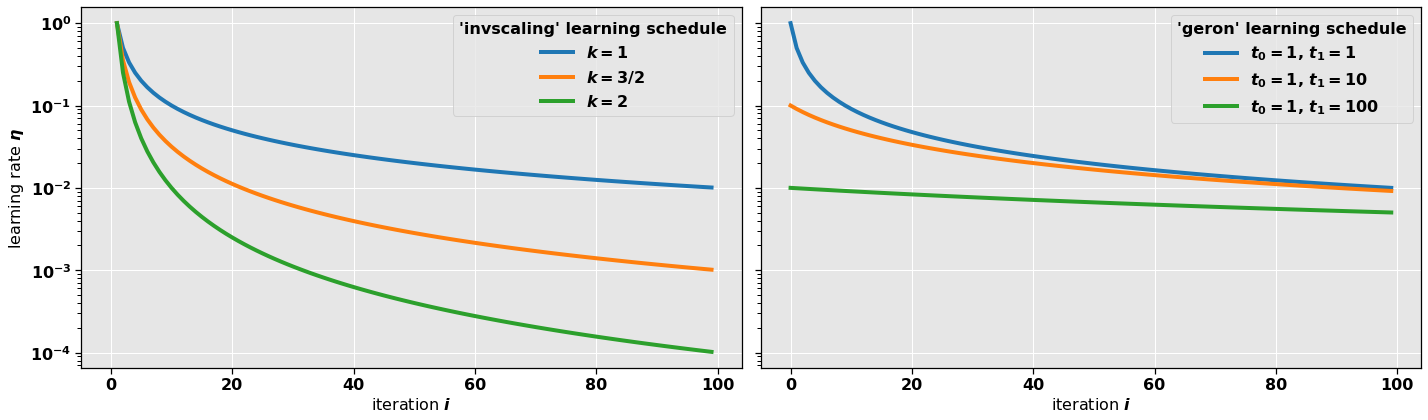
\includegraphics[width=1\linewidth]{learning_schedules.png}
	\caption{Two different learning schedules over the 100 first iterations. To the left we see the \lstinline|invscaling| schedule in Python's \lstinline|scikit-learn| module, as given in Equation (\ref{invscaling}). To the right we see the simple schedule suggested by Geron, as given in Equation (\ref{geron}).}
	\label{fig:learning_schedules}
\end{figure}

\begin{lstlisting}[caption={Stochastic Gradient Descent algorithm. Cost function gradients and learning schedules may be defined independently of the implementation of SGD. This implementation runs for \lstinline|epochs*batches| iterations, and does not sense if or when it converges.},label={lst:sgd}] [!ht]
	// Declarations
	betas = "initial coefficient values"
	epochs = "number of runs through data set"
	batches = "number of mini batches"
	iteration_number = 0

	// SGD process	
	FOR i = 1...epochs DO
		shuffle(data, targets)
		FOR j = 1...batches DO
			data_batch, targets_batch = "draw mini batch from full set w/o replacement"
			iteration_number++
			eta = learning_schedule(iteration_number, args...)
			grad = cost_function_gradient(data_batch, targets_batch)
			betas = betas - eta*grad
		END FOR
	END FOR
\end{lstlisting}


%of the of size $m = n/M$, 


\subsection{Logistic Regression}

\subsection{Feed-Forward Neural Network}

\clearpage
\section{Results} \label{results}
% - Present your results
% - Give a critical discussion of your work and place it in the correct context.
% - Relate your work to other calculations/studies
% - An eventual reader should be able to reproduce your calculations if she/he wants to do so. All input variables should be properly explained.
% - Make sure that figures and tables should contain enough information in their captions, axis labels etc so that an eventual reader can gain a first impression of your work by studying figures and tables only.

\subsection{Stochastic Gradient Descent: Linear Regression}


\subsection{Stochastic Gradient Descent: Logistic Regression}


\subsection{Feed-Forward Neural Network: Regression}


\subsection{Feed-Forward Neural Network: Classification}



\clearpage
\section{Discussion and Conclusion} \label{conclusion}
% - State your main findings and interpretations
% - Try as far as possible to present perspectives for future work
% - Try to discuss the pros and cons of the methods and possible improvements

\clearpage
\bibliographystyle{unsrt}
\bibliography{project2.bib}
\end{document}
